\documentclass[12pt,a4paper]{article}
\usepackage[utf8]{inputenc}
\usepackage[spanish,es-tabla]{babel}
\usepackage{geometry}
\usepackage{graphicx}
\usepackage{multirow}
\usepackage{tabularx}
\usepackage{mathptmx}
\usepackage{fancyhdr}
\usepackage{array}
\usepackage[table]{xcolor}
\usepackage{titlesec}
\usepackage{setspace}
\usepackage{microtype}
\usepackage{lastpage}
\usepackage{booktabs}
\usepackage{enumitem}
\usepackage{amsmath}
\usepackage{amsfonts}
\usepackage{amssymb}
\usepackage{listings}

\lstset{
  basicstyle=\ttfamily\footnotesize,
  breaklines=true,
  frame=single,
  numbers=none,
  backgroundcolor=\color{gray!5},
  showstringspaces=false
}

\graphicspath{{images/}{../images/}{../../images/}{./}}

\geometry{
    top=4.7cm,
    bottom=2.5cm,
    left=2.5cm,
    right=2.5cm,
    headheight=3.9cm,
    headsep=0.4cm
}

\setstretch{1.15}
\setlength{\parindent}{0pt}
\setlength{\parskip}{0.45em}
\setlength{\tabcolsep}{4pt}

\titleformat{\section}
  {\normalfont\fontsize{12}{14.5}\bfseries}{\thesection.}{0.6em}{\uppercase}
\titlespacing*{\section}
  {0pt}{1.8ex plus 0.4ex minus 0.2ex}{0.6ex plus 0.2ex}

\titleformat{\subsection}
  {\normalfont\fontsize{11.5}{13.5}\bfseries}{\thesubsection.}{0.5em}{}
\titlespacing*{\subsection}
  {0pt}{1.4ex plus 0.3ex minus 0.1ex}{0.4ex plus 0.1ex}

\titleformat{\subsubsection}
  {\normalfont\fontsize{10.5}{12.5}\bfseries\itshape}{\thesubsubsection.}{0.4em}{}
\titlespacing*{\subsubsection}
  {0pt}{1.1ex plus 0.2ex minus 0.1ex}{0.3ex plus 0.1ex}

\newcolumntype{Y}{>{\centering\arraybackslash}X}
\newcolumntype{L}{>{\raggedright\arraybackslash}X}
\newcolumntype{C}{>{\centering\arraybackslash}X}

\definecolor{headerred}{RGB}{180, 0, 0}
\definecolor{darkred}{RGB}{140, 0, 0}
\definecolor{lightgraybg}{RGB}{248, 248, 248}
\definecolor{tableheader}{RGB}{232, 238, 246}

\newcommand{\docCodigo}{TI-SIGE-ENT-S4-003}
\newcommand{\docVersion}{2.0}
\newcommand{\docProceso}{DESARROLLO BACKEND / CRIPTOGRAFÍA Y FIRMA ELECTRÓNICA}
\newcommand{\docElaboracion}{16/09/2026}
\newcommand{\docRevision}{APROBADO POR LÍDER TÉCNICO}
\newcommand{\docTitulo}{ENDPOINTS DE PERSISTENCIA Y API DE FIRMAS EN CASCADA (EXPRESS V5 / PG 18)}
\newcommand{\docOrganizacion}{FACULTAD DE INGENIERÍA EN SISTEMAS, ELECTRÓNICA E INDUSTRIAL}
\newcommand{\docSubOrganizacion}{CARRERA DE INGENIERÍA DE SOFTWARE}

\newcommand{\encabezadofrecuente}{%
    \renewcommand{\arraystretch}{1.15}%
    \noindent\makebox[\textwidth][c]{%
    \begin{tabularx}{\textwidth}{|>{\centering\arraybackslash}m{2.8cm}|Y|>{\centering\arraybackslash}m{4.8cm}|}
        \hline
        \multirow{4}{2.8cm}{\centering\raisebox{-1.15cm}{
\includegraphics[width=2.5cm,height=2.0cm,keepaspectratio]{images/logo.png}}}
        & \textbf{\fontsize{9}{11}\selectfont \docOrganizacion} 
        & \textbf{\fontsize{8}{10}\selectfont CÓDIGO:} \fontsize{8}{10}\selectfont \docCodigo \\
        \cline{3-3}
        & \textbf{\fontsize{8.5}{10.5}\selectfont \docSubOrganizacion} 
        & \textbf{\fontsize{8}{10}\selectfont VERSIÓN:} \fontsize{8}{10}\selectfont \docVersion \\
        \cline{2-3}
        & \textbf{\fontsize{8}{10}\selectfont PROCESO:} \fontsize{8}{10}\selectfont \docProceso 
        & \textbf{\fontsize{8}{10}\selectfont ELABORACIÓN:} \fontsize{8}{10}\selectfont \docElaboracion \\
        \cline{2-3}
        & \textbf{\fontsize{8.5}{10.5}\selectfont \docTitulo} 
        & \textbf{\fontsize{8}{10}\selectfont ÚLTIMA REVISIÓN:} \fontsize{8}{10}\selectfont \textbf{\textcolor{darkred}{\docRevision}} \\
        \hline
    \end{tabularx}%
    }%
}

\pagestyle{fancy}
\fancyhf{}
\fancyhead[C]{\encabezadofrecuente}
\fancyfoot[C]{\fontsize{10}{12}\selectfont Página \thepage\ de \pageref{LastPage}}
\renewcommand{\headrulewidth}{0pt}

\begin{document}

% =============================================================
% 1. TÍTULO
% =============================================================
\section{Título}
\textbf{Denominación del Entregable:} Especificación e Implementación de la API REST Modular: Persistencia Atómica en PostgreSQL 18 y Cascada de Firmas Electrónicas con Sellado SHA-256 (Node.js + Express v5 / FirmaEC PKCS\#12)



% =============================================================
% 2. INTRODUCCIÓN
% =============================================================
\section{Introducción}
La legalización de los documentos del Sistema de Gestión de la Calidad (SGC) en la FISEI UTA requiere una estricta validez jurídica y probatoria, en total apego a la Ley de Comercio Electrónico, Firmas Electrónicas y Mensajes de Datos del Ecuador. En el modelo manual tradicional, los expedientes en Word sufrían demoras de semanas entre firmas sucesivas por correo electrónico, desórdenes en la secuencia reglamentaria e incluso modificaciones no autorizadas post-aprobación.

Para erradicar definitivamente estas vulnerabilidades, el sistema \textbf{SIGE} implementa en su backend \textbf{Node.js + Express (v5)} un subsistema modular de \textbf{Persistencia Atómica y Cascada de Firmas Electrónicas compatible con FirmaEC (MINTEL) y certificados PKCS\#12 / token e-Token}. Mediante transacciones ACID en \textbf{PostgreSQL (18)} y sellado criptográfico mediante funciones de hash \textbf{SHA-256}, este módulo garantiza que cada documento avance por tres escalones jerárquicos inmutables y estrictamente secuenciales:
\begin{enumerate}[leftmargin=1.5em, itemsep=1.5pt]
    \item \textbf{Escalón 1: Elaborado por (Docente Responsable)}
    \item \textbf{Escalón 2: Revisado por (Coordinador del Área de Conocimiento)}
    \item \textbf{Escalón 3: Aprobado por (Coordinador de la Carrera de Software)}
\end{enumerate}

Ningún escalón puede firmar si el anterior no ha registrado un sello digital válido y comprobado contra la base de datos relacional.

% =============================================================
% 3. OBJETIVO
% =============================================================
\section{Objetivo}

\subsection{Objetivo General}
Desarrollar y documentar los endpoints de persistencia de documentos y la API de Firmas Electrónicas en Cascada en Node.js y Express (v5) con PostgreSQL (18), garantizando el principio de no repudio, la inmutabilidad documental y el cumplimiento del flujo jerárquico del SGC de la FISEI.

\subsection{Objetivos Específicos}
\begin{itemize}[leftmargin=1.5em, itemsep=1.5pt, topsep=1.5pt]
    \item Diseñar la arquitectura modular del backend: \texttt{documents.controller.js}, \texttt{documents.service.js} y \texttt{documents.repository.js} con soporte para transacciones ACID mediante \texttt{pg.Pool}.
    \item Implementar los endpoints de firma electrónica multinivel: \texttt{POST /api/documentos/:id/firmar-docente}, \texttt{POST /api/documentos/:id/firmas/coordinador-area} y \texttt{POST /api/documentos/:id/firmas/coordinador-carrera}.
    \item Integrar la verificación determinista de precondiciones de Validation Gates (100.00\% de ponderaciones en la matriz del Plan; 100\% de evidencias en el Informe) previa a la generación del resumen criptográfico SHA-256.
    \item Registrar el sello digital en Base64, el número de serie del certificado X.509 y el timestamp UTC en la tabla \texttt{firmas\_legalizacion}.
\end{itemize}

% =============================================================
% 4. ALCANCE
% =============================================================
\section{Alcance}

\subsection{Alcance Incluido}
Operaciones CRUD completas para borradores de planes e informes, endpoints de persistencia de secciones descriptivas (\texttt{PUT /api/documentos/:id/secciones}), transición y bloqueo de edición en PostgreSQL 18, generación de resumen hash SHA-256 y registro inmutable en \texttt{auditoria\_sistema}.

\subsection{Límites y Exclusiones}
No sustituye la infraestructura de clave pública (PKI) de las entidades de certificación autorizadas ni custodia contraseñas de certificados \texttt{.p12} en la base de datos.

% =============================================================
% 5. DEFINICIONES
% =============================================================
\section{Definiciones}
\begin{itemize}[leftmargin=1.5em, itemsep=2pt, topsep=2pt]
    \item \textbf{FirmaEC:} Aplicativo oficial de firma digital desarrollado por el MINTEL para estampar firmas digitales X.509 en Ecuador.
    \item \textbf{PKCS\#12 (.p12):} Formato estándar de archivo que almacena certificados criptográficos y claves privadas protegidas por contraseña.
    \item \textbf{Cascada de Firmas:} Flujo procedimental jerárquico donde la firma subsiguiente depende de la preexistencia y validez de la firma previa.
    \item \textbf{Sello Digital Base64:} Representación textual codificada de la firma criptográfica generada sobre el hash SHA-256 del documento.
    \item \textbf{EDT (\textit{Estructura de Desglose del Trabajo}):} Descomposición funcional jerárquica de entregables del proyecto.
\end{itemize}

% =============================================================
% 6. RESPONSABILIDADES
% =============================================================
\section{Responsabilidades}
\begin{itemize}[leftmargin=1.5em, itemsep=2pt, topsep=2pt]
    \item \textbf{Nixon Hurtado (Backend Developer / DBA):} Implementación de controladores, servicios y repositorios en Express (v5) y transacciones en PostgreSQL 18.
    \item \textbf{Steeven Toala (Líder / Arquitecto):} Diseño del protocolo criptográfico, hashing SHA-256 e integración con FirmaEC.
    \item \textbf{Andrea Vasquez (Frontend / QA):} Consumo de endpoints mediante cliente Axios con auto-renovación y pruebas de flujo.
    \item \textbf{Ing. Paulo Torres (Docente Tutor):} Validación de apego a la normativa SGC de la UTA y aprobación del circuito.
\end{itemize}

% =============================================================
% 7. NORMATIVA LEGAL Y TÉCNICA
% =============================================================
\section{Normativa Legal y Técnica}
\begin{itemize}[leftmargin=1.5em, itemsep=2pt]
    \item \textbf{Ley de Comercio Electrónico del Ecuador:} Art. 14 (Efectos jurídicos) y Art. 15 (Requisitos de validez probatoria).
    \item \textbf{Estándar CMS / PKCS\#7 (RFC 5652):} Sintaxis de mensajes criptográficos para firmas digitales.
    \item \textbf{OWASP API Security Top 10 (2023):} Mitigación de Broken Object Level Authorization (API1) y Broken Function Authorization (API5).
\end{itemize}

% =============================================================
% 8. MÉTODO, POLÍTICAS Y CONTENIDOS
% =============================================================
\section{Método, Políticas y Contenidos}
El flujo jerárquico de firmas se rige por políticas criptográficas deterministas: se genera el hash inmutable SHA-256 del documento una vez verificado el 100.00\% de ponderaciones en el plan o el 100\% de evidencias en MinIO S3 para el informe. Cada escalón firma de forma secuencial e inmutable.

\begin{figure}[htbp]
    \centering
    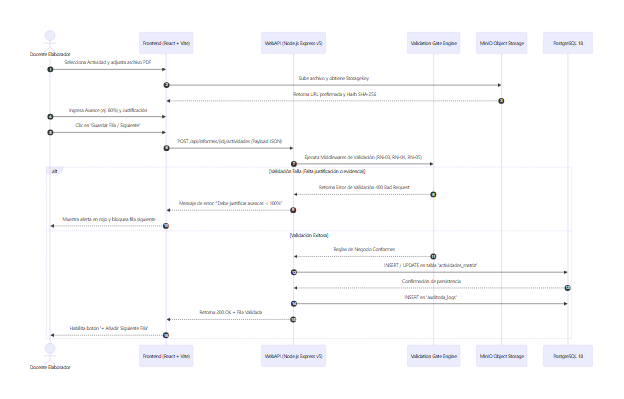
\includegraphics[width=0.88\textwidth,keepaspectratio]{images/s2_03_secuencia_validation.png}
    \caption{Interacción Criptográfica con FirmaEC y Registro en PostgreSQL 18.}
    \label{fig:secuencia_firmaec}
\end{figure}

% =============================================================
% 9. DESCRIPCIÓN DE ACTIVIDADES
% =============================================================
\section{Descripción de actividades}

\subsection{Especificación de los Endpoints REST de Firmas}
Se definieron tres compuertas secuenciales protegidas por roles RBAC:

\begin{table}[htbp]
\centering
\small
\renewcommand{\arraystretch}{1.2}
\begin{tabularx}{\textwidth}{|l|X|l|X|}
\hline
\rowcolor{tableheader}
\textbf{Método y Ruta} & \textbf{Precondición Estricta} & \textbf{Orden} & \textbf{Transición de Estado} \\
\hline
\texttt{POST .../firmar-docente} & Ponderación matriz == 100.00\% & 1 (Docente) & PLAN\_PENDIENTE\_FIRMA\_COORD\_AREA \\
\hline
\texttt{POST .../firmas/coordinador-area} & Existe Firma 1 con estado FIRMADO & 2 (Área) & PLAN\_PENDIENTE\_FIRMA\_COORD\_CARRERA \\
\hline
\texttt{POST .../firmas/coordinador-carrera} & Existe Firma 2 con estado FIRMADO & 3 (Carrera) & PLAN\_APROBADO\_Y\_LEGALIZADO $\rightarrow$ EN\_EJECUCION \\
\hline
\end{tabularx}
\caption{Matriz de Endpoints y Compuertas de Cascada de Firmas.}
\end{table}

\subsection{Implementación del Endpoint de Firma en Express v5}
\begin{lstlisting}[language=Java]
// backend/src/modules/documents/documents.controller.js
import crypto from 'crypto';
import pool from '../../config/db.js';

export const firmarPlanDocente = async (req, res, next) => {
  const client = await pool.connect();
  try {
    const { id } = req.params;
    const { selloDigitalBase64, serialCertificado } = req.body;
    const userId = req.user.sub;
    await client.query('BEGIN');

    const docRes = await client.query('SELECT * FROM documentos WHERE id = $1', [id]);
    const doc = docRes.rows[0];
    if (!doc) throw new Error('Documento no encontrado');

    const matRes = await client.query(
      'SELECT COALESCE(SUM(ponderacion), 0) AS total FROM actividades_matriz WHERE documento_id = $1',
      [id]
    );
    const total = parseFloat(matRes.rows[0].total);
    if (Math.abs(total - 100.0) > 0.01) {
      throw new Error(`Invariante violada: Suma de ponderaciones es ${total}%, debe ser 100%`);
    }

    const hash = crypto.createHash('sha256').update(`${doc.id}:${doc.version_actual}`).digest('hex');
    await client.query(
      `INSERT INTO firmas_legalizacion (documento_id, usuario_firmante_id, fase_documento,
       orden_cascada, rol_instancia, estado_firma, serial_certificado, sello_digital_base64, hash_documento)
       VALUES ($1, $2, 'PLAN_TRABAJO', 1, 'DOCENTE_RESPONSABLE', 'FIRMADO', $3, $4, $5)`,
      [id, userId, serialCertificado || 'CERT-UTA-001', selloDigitalBase64 || 'SELLO_B64', hash]
    );

    await client.query(
      "UPDATE documentos SET estado_actual = 'PLAN_PENDIENTE_FIRMA_COORD_AREA', updated_at = NOW() WHERE id = $1",
      [id]
    );
    await client.query('COMMIT');
    res.json({ success: true, message: 'Plan legalizado por docente' });
  } catch (err) {
    await client.query('ROLLBACK');
    next(err);
  } finally { client.release(); }
};
\end{lstlisting}

\subsection{Conclusiones y Recomendaciones Técnicas}
\begin{itemize}[leftmargin=1.5em, itemsep=2pt]
    \item El API de Firmas Electrónicas en Cascada elimina la posibilidad de firmas extemporáneas, asincronías reglamentarias o fraudes documentales en el SGC de la FISEI.
    \item La compatibilidad nativa con certificados X.509 de FirmaEC y la trazabilidad en PostgreSQL 18 otorgan plena validez jurídica a los planes e informes generados.
    \item Realizar pruebas de carga en el endpoint de cálculo de hashes para expedientes con múltiples evidencias adjuntas.
\end{itemize}

\vspace{0.3cm}

% =============================================================
% 10. FIRMAS DE RESPONSABILIDAD
% =============================================================
\section{Firmas de Responsabilidad}

\noindent
\renewcommand{\arraystretch}{1.2}
\begin{tabularx}{\textwidth}{|>{\raggedright\arraybackslash}m{2.9cm}|>{\raggedright\arraybackslash}X|>{\centering\arraybackslash}m{4.6cm}|>{\centering\arraybackslash}m{2.3cm}|}
    \hline
    \rowcolor{headerred}
    \textcolor{white}{\textbf{ACCIÓN}} & \textcolor{white}{\textbf{NOMBRE Y CARGO}} & \textcolor{white}{\textbf{FIRMA}} & \textcolor{white}{\textbf{FECHA}} \\
    \hline
    \textbf{Elaborado por:} & Nixon Hurtado\newline \textit{Backend Developer / DBA} & \parbox[c]{4.4cm}{\centering\vspace{10pt}\textbf{\textcolor{blue!80}{\scriptsize [ FIRMADO DIGITALMENTE ]}}\vspace{10pt}} & 16/09/2026 \\
    \hline
    \textbf{Revisado por:} & Steeven Toala\newline \textit{Líder de Proyecto / Arquitecto Software} & \parbox[c]{4.4cm}{\centering\vspace{4pt}
\includegraphics[height=1.5cm,width=4.0cm,keepaspectratio]{images/firma_steveen.png}\vspace{4pt}} & 16/09/2026 \\
    \hline
    \textbf{Aprobado por:} & Ing. Paulo Torres\newline \textit{Docente Tutor - Gestión Proyectos Software} & \parbox[c]{4.4cm}{\centering\vspace{10pt}\textbf{\textcolor{gray!80}{\scriptsize [ PENDIENTE DE APROBACIÓN ]}}\vspace{10pt}} & \textbf{\textcolor{gray!90}{Pendiente}} \\
    \hline
\end{tabularx}

\vspace{0.4cm}

% =============================================================
% 11. CONTROL DE CAMBIOS
% =============================================================
\section{Control de Cambios}

\noindent
\renewcommand{\arraystretch}{1.2}
\begin{tabularx}{\textwidth}{|>{\hsize=0.45\hsize\centering\arraybackslash}X|>{\hsize=1.55\hsize\raggedright\arraybackslash}X|>{\hsize=1.2\hsize\raggedright\arraybackslash}X|>{\hsize=0.8\hsize\centering\arraybackslash}X|}
    \hline
    \rowcolor{gray!20}
    \textbf{Versión} & \textbf{Descripción del cambio} & \textbf{Responsable del cambio} & \textbf{Fecha de aprobación} \\
    \hline
    1.0 & Especificación inicial de compuertas de firma. & Nixon Hurtado & 16/09/2026 \\
    \hline
    2.0 & Actualización integral al stack oficial: Node.js + Express (v5) modular, transacciones ACID en PostgreSQL 18, sellado SHA-256 e integración con FirmaEC. & Nixon Hurtado / Steeven Toala & 16/09/2026 \\
    \hline
\end{tabularx}

\vspace{0.4cm}

% =============================================================
% 12. ANEXOS
% =============================================================
\section{Anexos}

\subsection*{Anexo 1: Referencias Bibliográficas}
\begin{itemize}[leftmargin=1.5em, itemsep=2pt]
    \item MINTEL. (2025). \textit{Guía de Integración Técnica del Aplicativo FirmaEC}. Quito, Ecuador.
    \item Express.js Team. (2026). \textit{Express 5.x Database Transactions with pg.Pool}.
    \item PostgreSQL Global Development Group. (2026). \textit{PostgreSQL 18 Documentation: Concurrency Control}.
\end{itemize}

\subsection*{Anexo 2: Resumen de Endpoints del API de Firmas}
\begin{itemize}[leftmargin=1.5em, itemsep=2pt]
    \item \texttt{POST /api/documentos/:id/firmar-docente}: Registro de firma escalón 1 (Docente).
    \item \texttt{POST /api/documentos/:id/firmas/coordinador-area}: Registro de firma escalón 2 (Coordinador Área).
    \item \texttt{POST /api/documentos/:id/firmas/coordinador-carrera}: Registro de firma escalón 3 (Coordinador Carrera).
\end{itemize}

\end{document}
